\documentclass{article}

\usepackage{graphicx}
\usepackage{lmodern}
\usepackage{enumitem}

\begin{document}
	\begin{titlepage}
		\fontfamily{pbk}\selectfont
		\hbox{			
			\rule{1pt}{\textheight}
			\hspace*{0.05\textwidth}
			\parbox[b]{\textwidth}{
				\Large Project Tender\\[1cm]
					
				\Huge Project: Property Investment Optimiser\\
				\huge Client: CSIR\\[0.8cm]					
					
				{\huge Team: HTTP\textunderscore418}
				
				\begin{itemize}[label={}, leftmargin=0pt, noitemsep]
					\Large						
					\item Christiaan Saaiman, 12059138
					\item Michael Loosen, 14017254
					\item Elizabeth Bode, 14310156
					\item LC Meyers, 14024633
				\end{itemize}
				\vspace{0.5cm}
					
				{\large Department of Computer Science, University of Pretoria\\[0.2cm]}

				\Large\today\\[0.3cm]				
									
				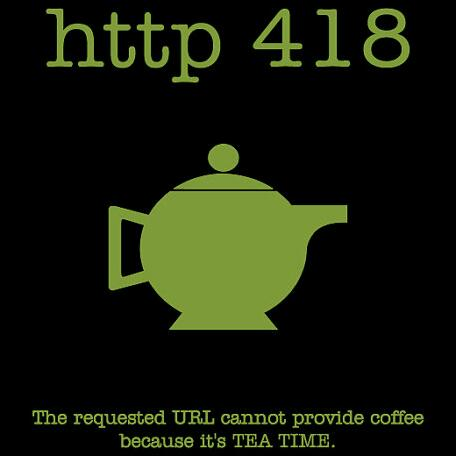
\includegraphics[scale=0.3]{../teamPic.jpg}					
			}								
		}
	\end{titlepage}
	\newpage
	\section{The Team}
	\subsection{LC Meyers}
	\begin{figure}[h]
		\centering
		
\includegraphics[height=0.3\textheight]{../charl.jpg}
	\end{figure}
	\begin{itemize}
		\item \textbf{Full name:} Lodewyk Charles Meyers
		\item \textbf{My interests:}
			\subitem Gaming
			\subitem Computers
			\subitem Music
			\subitem User experience design
			\subitem Website design
			\subitem Anything new related to technology
		\item \textbf{My technical skills:}
			\subitem Web development skills
			\subitem Database design
			\subitem Java
			\subitem C\#
		\item \textbf{Past experience that might help:}
			\subitem I collaborated on a website for a school as part of a project.			
		\item \textbf{Non-technical strenghts:}
			\subitem I have a high amount of patience
			\subitem Hardworking
			\subitem Eager to learn new things
			\subitem Enjoy trying to solve complex problems
		\item \textbf{What makes me want to do this project?} I love web development and will enjoy this project a lot. I still want to learn how to use C\# for a web server and web based development and this project will be the perfect opportunity for me to learn C\# web based development.
	\end{itemize}
	
	\section{Project excecution}
		\subsection{Technologies we will use for the project:}
		\begin{itemize}
			\item For the front end we will use Bootstrap framework along with JQuery to handle AJAX requests to the server. Bootstrap makes making responsive websites very easy, thus the choice in Bootstrap.
			\item For the backend we will use C\# for the RESTful web server to serve the results of calculations to the client. If needed we can also use C\# for the front end of the system.	
		\end{itemize}
\end{document}